% Background chapter continued..

\section{Similarity Methods}
\label{similarity_methods}
There are several methods available to calculate similarity score.
\\

\subsection{Cosine Similarity}
\label{cosine_similarity}
In cosine similarity measure \cite{19}, the result is the cosine of the angle between two vectors. It is measured by the cosine angle between two vectors and discovers the direction between two vectors is same or not. Often it is used to calculate document similarity in text analysis. The item ratings or preferences are stored in one vector called as item vector. The preferences of user are stored in another vector based on user's ratings and likes-dislikes is known as profile vector. Consider $A = (5,0,3,0,2)$ and $B = (3,0,2,0,2)$ are profile vector and item vector respectively, the similarity between them can be calculated as per \autoref{eq:cosine_similarity}.
\\

\begin{equation}
sim(A,B) = cos(\theta) = \frac {A.B}{\parallel A \parallel \parallel B \parallel} = \frac{\sum_{i=1}^{n} {A_{i} B_{i}}}{\sqrt{\sum_{i=1}^{n} {A_{i}^2}} \sqrt{\sum_{i=1}^{n} {B_{i}^2}}}
\label{eq:cosine_similarity}
\end{equation}

\begin{figure}[H]
	\centering
	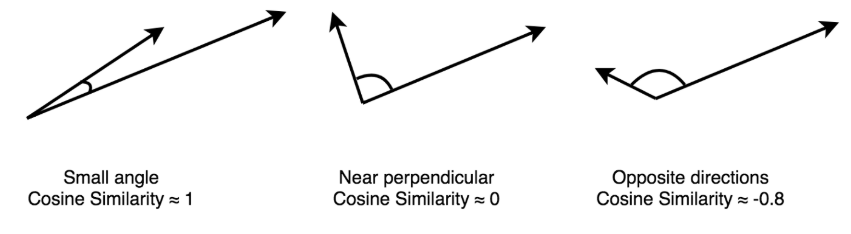
\includegraphics[width=0.7\linewidth]{cosine_similarity}
	\caption{Cosine Similarity}
	\label{fig:cosine_similarity}
\end{figure}

\noindent
Using \autoref{cosine_similarity} if we compute cosine similarity between A and B vectors, then we get:
\begin{align*}
\parallel A \parallel \parallel B \parallel &=(5 x 3 + 0 x 0 + 3 x 2 + 0 x 0 + 2 x 2  ) = 25 \\
\parallel A \parallel  &= \sqrt{5^2 + 0^2 + 3^2 + 0^2 + 2^2}  = 6.164414 \\	     
\parallel B \parallel  &= \sqrt{3^2 + 0^2 + 2^2 + 0^2 + 2^2}  = 3.74165\\	     
sim(A,B)  &=  0.92 
\end{align*}
\noindent The value of cosine angle ranges between -1 to 1. Calculated result 0.92 shows that vector A and B are quite similar as the result inclines towards 1. As we can see in \autoref{fig:cosine_similarity} lesser the angle, less distance between vectors hence vectors considered as more similar to each other.
\\
\subsection{Euclidean Distance Similarity}
\label{euclidean_distance}
The Euclidean distance between two points is the length which is connecting those two points. If we plot n dimensional space and plot similar items, then they will fall under close proximity. Consider a example of a positive quadrant of space and we plot items on the axis which are rated by user. The \autoref{user_movie_rating_table} illustrates the relationship between users and movies with ratings. The points drawn on graph in \autoref{fig:movie_plots} represents rating given by the user to those particular movies.

\begin{table}[]
\centering
\begin{tabular}{|l|l|l|l|}
\hline
Movie/User & Lady in the water & Snakes on a plane & You Me and Dupree \\ \hline
A          & 2.5               & 3.5               & 2.5               \\ \hline
B          & 3                 & 3.5               & 3.5               \\ \hline
C          & 2.5               & 3                 &                   \\ \hline
D          &                   & 3.5               & 2.5               \\ \hline
E          & 3                 & 4                 & 2                 \\ \hline
F          & 3                 & 4                 & 3.5               \\ \hline
G          &                   & 4.5               & 1                 \\ \hline
\end{tabular}
\caption{User-Movie Rating Relationship \cite{11}}
\label{user_movie_rating_table}
\end{table}

\begin{figure}[H]
	\centering
	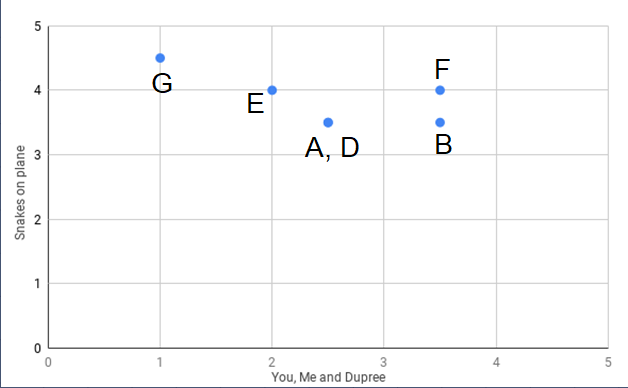
\includegraphics[width=0.7\linewidth]{movie_plots}
	\caption{Movie Rating Plots \cite{11} } 
	\label{fig:movie_plots}
\end{figure}

\noindent In that case, we can calculate distance between items with Euclidean distance formula which is given by \autoref{euclidean_distance}
\\
\begin{equation}
\textrm{Euclidean Distance } = \sqrt{(x_1 - y_1)^2 + ... + (x_n - y_n)^2}
\label{euclidean_distance}
\end{equation}

\noindent From above example, if we calculate Euclidean's distance between user A and user B then we get :
\begin{align*}
Distance (A, B) &= \sqrt{(3.5 - 3.5)^{2} + (3.5 - 2.5)^{2}} \\
\textrm{Similarity score }(A,B) &= \frac{1}{1+ Distance} = 0.5
\end{align*}


\subsection{Pearson's Correlation Similarity}
\label{pearson_correlation}
Person's correlation helps in finding correlation between two users or items. Correlation values ranges from -1 to 1 \cite{20}. Correlation on higher side implies more similarity. \autoref{eq:pearson_corr} gives correlation between two users $r_{u}$ and $r_{v}$.

\begin{equation}
sim(u,v) = \frac{\sum (r_{ui} - \bar{r}_u) (r_{vi} - \bar{r}_v )}{\sqrt{(\sum (r_{ui} - \bar{r}_u))^2} \sqrt{(\sum (r_{vi} - \bar{r}_v )^2}}
\label{eq:pearson_corr}
\end{equation}

\noindent Where $r_{ui}$ and $r_{vi}$ are rating scores for from two users. $\bar{r_{u}}$ and $\bar{r_{v}}$ denote the average rating by the two users.
Pearson correlation score $> 0$ indicates positive association. On the other hand, Pearson correlation score $ < 0$ indicates the negative correlation and score $ = 0$ indicates that no correlation. Hence a correlation value can capture a rating similarity between two users.
